\chapter{Getting Ready to Get Tactical}


\includegraphics[scale=0.20]{../images/ingredients-498199_1920.jpg}

\justify
Think of this chapter as the \emph{mise en place} of our DevSecOps souffle. 

\pagebreak
\justify
Let's start our preparations by outlining our overall objectives. We want to:
\justify
\begin{itemize}
\item
  Create an extensible lab environment for rapid prototyping and
  development. Get out of our old comfort zone, into a new one.
\item
  Keep our lab costs down while meeting the rest of the objectives.
  Utilize free services and open source tools to the extent possible.
\item
  Use the published best practices for each tool we choose to employ.
\item
  Always leave our project in a functional state.
\end{itemize}

\justify
The ideas captured here are not means to any end. Rather, these are meant to be
starting points, giving you a frame of reference with novel technologies and techniques
that will streamline your workflows and give your projects a productivity boost.
The hope is the reader will gain momentum to pursue these new ideas by following
along with the examples outlined in this book.

\justify
You should work to build up a solid base of code examples and problem solving
techniques that will greatly increase your efficacy. Over time, new tools and
processes will rotate in and out of your toolbox as technology progresses. Keep
in mind that your job is to maintain that momentum, to keep experimenting and
to see what is useful enough to stick with you and make a permanent part of your
repertoire.

\justify
Companies often make their services free in the hopes that you will see the value and usefulness of their products. The thinking goes that hopefully you will see enough utility that you will recommend them to your enterprise clients and integrate their products into your workflows. Not a bad trade-off! It only makes sense to avail yourself of free-tier cloud services, build and test platforms, and low or no-cost hosting environments. There are plenty of these out there and we will explore some of these as we dive further into the topics.

\justify
When we choose to use a tool, say Ansible for example, it only makes sense to also adopt the most up-to-date and best practices for using that tool. File system layout, naming conventions, script syntax and organization, and so on. We get to enjoy the clear and safe path forged by the folks that came before us, and with whom we share many goals. As your skills mature over time, you may want to consider donating time back to the open source and other communities upon which your knowledge has been built.

\justify
Finally, I find it very helpful for my own personal peace of mind to leave projects clean and green, to the extent possible. In other words, there is mental benefit to tidying up your physical and virtual workspace before walking away from the keyboard for the day. Perhaps you would find similar benefit should you choose to adopt this practice.

\section{Prerequisites}

\justify
This book intends to be a practical treatment of common and popular technologies
from the DevSecOps world. As such, we assume the reader has some basic knowledge
of certain concepts. We will be exploring new ways
of working for folks who are somewhat familiar with:

\begin{itemize}
\item
  Linux (UI and command line)
\item Python 3
\item
  Familiarity with github.com and the concepts of pull requests and branching.
\end{itemize}

\justify
The examples in this book have been tested on Linux running the latest
version of Docker.

\justify
Let's take a look at some of the other foundational environmental
elements we need in place to be successful.

\subsection{Windows Specific Prerequisites}

\begin{itemize}
\item installation of power shell
\item installation of python 3.9.x
\item installation of gh or github command line client
\end{itemize}

\subsection{Linux Specific Prerequisites}
\justify
When installing Docker on Linux hosts, it should be noted that docker-compose must be installed separately.

\section{The Workhorse (IDE)}
\justify
It is quite helpful to have a piece of software on your workstation that
makes code creation and edits easier. This software is commonly known as
an Integrated Development Environment (IDE)\index{IDE}.

\justify
One of the key features to look for in an IDE is to use one that you
don't have to spend a lot of time configuring and maintaining. A decent
IDE with the right add-ons can provide syntax highlighting to show
potential issues you might have missed, help you check for spelling or
grammar mistakes in your documentation, and even makes suggestions on
alternate ways of writing your code.

\justify
Visual Studio Code\footnote{\url{https://code.visualstudio.com/Download}}
from Microsoft is quite a popular choice these days in a large sea of
commercial and Open Source candidates. VSCode\index{VSCode} works well on Linux, Mac
and other operating systems. The environment is easily extensible to
support most any language, linter, or syntax checker we may have a need
for, thanks to their easy to use and well integrated "Extensions"
feature. VSCode also has an integrated terminal window\index{Terminal Window} so the developer
can execute shell commands without leaving the IDE screen.
 
\justify
Folks also seem to be quite fond of the Sublime\footnote{\url{https://www.sublimetext.com/}} IDE for similar reasons, including it's customizability and extensibility.

single: Sublime

\begin{figure}
\centering
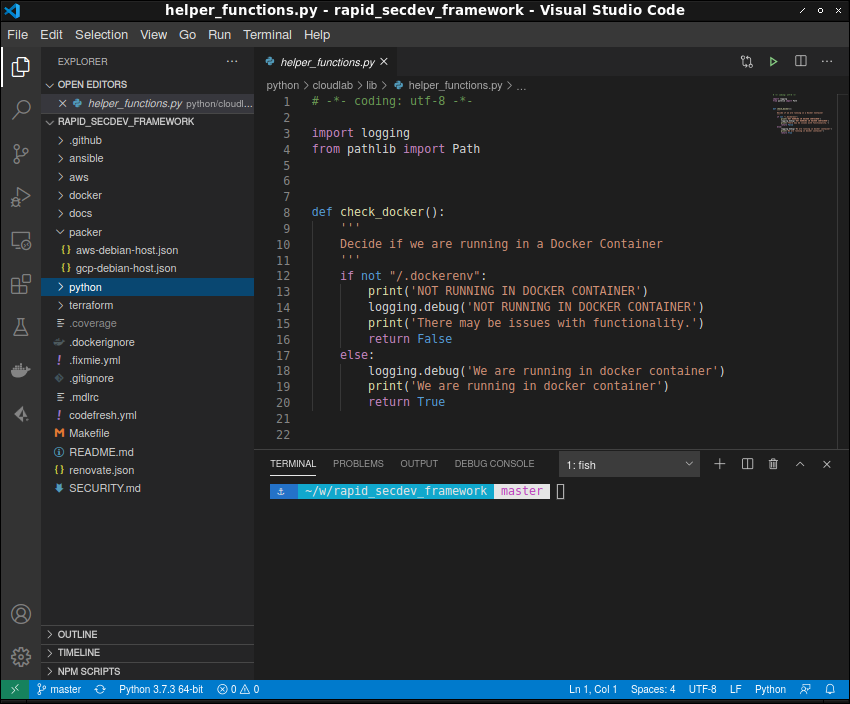
\includegraphics[scale=0.45]{../images/setup-vscode.png}
\caption{The VScode IDE.}
\end{figure}

\section{Lab Exercises}
\justify
This book is meant to be a workbook as much as it is meant to be read. You are encouraged to jump ahead, go back and re-read, do the exercises you think you can apply the learning objective from right away, and skip the parts you don't think you will ever use. Learning can be a non-linear experience and you are encouraged to "color outside the lines" to the extent you feel comfortable doing so.

\justify
That said, I've attempted to give this book a feel of moving the reader along towards a final project. This project is meant to guide the reader through applying the information introduced between this chapter and that.
